
\documentclass [french]{sig-alternate-05-2015}
\usepackage{color}
\usepackage[francais]{babel}
\usepackage[utf8]{inputenc}
\usepackage{lmodern}
\usepackage[noend]{algpseudocode}
\usepackage{subcaption}
\usepackage{subfig} 
\usepackage{graphicx}
\usepackage[rflt]{floatflt}
\usepackage{mathrsfs}
\usepackage{multirow}
\usepackage{array}
\usepackage[rflt]{floatflt}
\usepackage{makecell}

\renewcommand\theadalign{cb}
\renewcommand\theadfont{\bfseries}
\renewcommand\theadgape{\Gape[3pt]}
\renewcommand\cellgape{\Gape[3pt]}

\begin{document}



\title{Expressive Virtual Storyteller for Children}



\numberofauthors{3} 
\author{
\alignauthor Lydia Ould Ouali\\
       \affaddr{LIMSI}\\
       \affaddr{rue John von Neumann}\\
       \affaddr{91405 Orsay }\\
       \email{ouldouali@limsi.fr}
% 5th. author
\alignauthor Nicolas Sabouret\\
       \affaddr{LIMSI}\\
       \affaddr{rue John von Neumann}\\
       \affaddr{91405 Orsay }\\
       \email{sabouret@limsi.fr}
        \and
% 6th. author
\alignauthor Charles Rich\\
       \affaddr{WPI}\\
       \affaddr{Worcester Polytechnic Institute}\\
       \affaddr{Worcester, MA, USA}\\
       \email{rich@wpi.com}    
}


\maketitle
\begin{abstract}

\end{abstract}


\keywords{Relation interpersonnelle;negociation coopérative, dialogue social}

\section{Introduction}
La modélisation d’agents conversationnels connaît un véritable essor dans différents domaines applicatifs où l'agent est muni d'un système de dialogue lui permettant de jouer différents rôles tels que  le rôle de compagnon \cite{sidner2013always} ou encore de conseiller \cite{bickmore2005s}. 

\par Les systèmes de dialogues existants peuvent être divisé en deux catégories; les systèmes de dialogue orienté tâches et les systèmes de dialogue sociaux. Les systèmes de dialogues orienté tâches sont les plus anciens, où les dialogues se centraient  exclusivement sur la collaboration avec l’utilisateur pour satisfaire des tâches communes \cite{allen1995spoken, allen1996robust}. Cependant, un certain nombre de recherches ont montré que l’aspect social ne peut être ignoré dans un dialogue, car ce dernier est social par définition \cite{markopoulos2005case}. Par ailleurs, \cite{moon1998intimate} a démontré que les utilisateurs préféraient interagir avec des agents dotés d'aptitudes sociales qui lui permettraient de construire une relation sur le long-terme avec l'utilisateur \cite{bickmore2005establishing}. Par conséquent, en plus des tâches à satisfaire, les chercheurs prennent en compte l'aspect social de la conversation dans la mise en œuvre de systèmes de dialogues. Ces derniers sont considérés comme des systèmes de dialogues sociaux.
 Néanmoins, il existe encore peu de recherches qui s’intéressent a une modélisation explicite et dynamique de la relation sociale entre l’agent et l’utilisateur (c.-à.-d. qui évolue au cours de l'interaction). Les travaux existants se sont limités à une modélisation qui vise a améliorer la collaboration de l’agent et l'utilisateur sur une interaction limitée dans le temps. Dans le cadre d'une interaction sur long-terme (voir section \ref{RW}), une modélisation explicite du comportement social de l’agent doit être considérée, car cette dernière influence le dialogue directement, en terme de contenue et de stratégies mises en place par l’agent pour satisfaire ses buts \cite{bickmore2012empirical}.

\par La modélisation des comportements sociaux a été largement étudiée en psychologie sociale, plusieurs travaux ont analysés les différentes dimensions qui peuvent affecter le comportement social dans le cadre d’une interaction humain/ humains. Ces notions peuvent être adaptées et utilisées pour le cas d’une interaction humain agent.

 \par \emph{Laver}\cite{laver1981linguistic} définit le dialogue social comme un processus d'échange de préférences et d'opinions sur un sujet de conversation. Cet échange de préférences peut conduire les interlocuteurs à mener une négociation - sur leurs préférences - afin de trouver un compromis qui arrangerait les deux participants. Par exemple, deux interlocuteurs qui cherchent un restaurant où dîner à Paris. Ce type de négociation est nommé \emph{négociation coopérative}. Nous pouvons donc considérer un dialogue social comme un processus de négociation coopérative sur les préférences, où les stratégies employées par les interlocuteurs pour présenter leurs préférences sont directement affectées par leurs perceptions de la relation interpersonnelle.

\par Dans cette optique, nous proposons dans ce papier d'étudier l'impact des relations interpersonnelles sur les stratégies de dialogue employées par interlocuteurs spécialement dans le cadre d'une négociation coopérative. L'article sera architecturé comme suit. La section \ref{RW} reprend les les travaux autours de notre thématique. La section \ref{contribution} sera dédiée à la présentation de notre modèle dialogique préliminaire ainsi que son implémentation. Les perspectives et futurs travaux seront discutés dans la section \ref{conc}.

\section{Travaux connexes}
\label{RW}
%Cette section sera dédié à l'état de l'art existant autour de notre thématique de thèse. nous présenterons les systèmes de dialogues qui s'intéressent à la modélisation des relations avec l'utilisateur, ainsi qu'une représentation des relations interpersonnelles.  
La modélisation d'un dialogue social consiste à concevoir un modèle de conversation où les buts interpersonnels sont mis en avant et les buts orienté tâches, s'ils existent, sont mis en arrière plan \cite{bickmore2005social}. {\color{red} Trouver la transition vers la négociation coopérative}
%Par exemple, une personne peut avoir l'intention d'impressionner son amie et va donc initier un dialogue avec un but  tâche de trouver un restaurant où elle aimerait dîner. 
Des travaux sur la négociation coopérative dans le dialogue existent déjà. Par exemple \cite{amgoud2000arguments, daskalopulu1998handling} qui ont mis en œuvre des modèles formels de dialogue où les agents sont capables de négocier et même d'argumenter sur leurs choix de préférences. Cependant, ces travaux négligent l'aspect social du dialogue dans la conception des stratégies de négociation. Cependant, il a été prouvé que les relations sociales affectent directement le comportement des interlocuteurs \cite{bickmore2000weather, bickmore2005establishing, moon1998intimate, nass2000does} et par conséquent leurs stratégies dans le dialogue. Par exemple, une personne dominante exprime facilement ses préférences et argumente contrairement a une personne soumise. 


\subsection{ACA sociaux}

\par Il existe dans la littérature des  ACA sociaux  qui arrivent à modéliser leurs relations avec l'utilisateur et la gérer afin d'adapter leur comportements dans la conversation. Nous citons trois principales contributions:

\par \textbf{Autom :} Le robot Autom \cite{kidd2005sociable} est conçu pour jouer le rôle d'un conseiller de perte de poids, placé dans les maisons des utilisateurs pour une intervention sur le long terme. Le robot s'intéresse principalement à trois facteurs de relations avec l'utilisateur, à savoir \textit{l'engagement, la confiance et la motivation}.  Le modèle de relation utilisé est construis sur trois étapes. La première étape est la prise de connaissance où le robot doit  d'abord encourager l'utilisateur à s'engager dans une interaction avec le système, pour ensuite le motiver à réaliser les tâches.
La seconde étape est la construction des relations avec l'utilisateur. En effet, le robot doit être explicite sur les avantages qu'il peut apporter à l'utilisateur, sa compréhension du système est obligatoire afin que l'utilisateur puisse construire une relation de confiance avec le robot qui permettra à ce dernier de répondre aux attentes de l'utilisateur.  La dernière étape est la maintenance de la relation qui est la partie la plus importante, où le robot doit s'assurer du maintient de l'engagement de l'utilisateur pour établir une relation de confiance au fil des interactions. Le système dispose  d'un nombre limité d'acte de langage afin d'établir et maintenir sa relation avec l'utilisateur.


\par \textbf{FitTrack: } est un des premiers systèmes à mener une étude longitudinale sur l'engagement entre l'utilisateur et un agent virtuel \cite{bickmore2005s}. Le cadre de l'étude consiste à changer les comportements de santé. L'agent joue le rôle d'un conseillé d'exercices avec qui les utilisateurs interagissent quotidiennement durant un mois. L'agent utilise un large éventail de techniques tirées de la psychologie sociale des relations, dont les communication personnelles méta-relationnelles, l'empathie, le dialogue social afin de construire un terrain d'entente, ainsi que la prise en compte des comportements non verbaux. Tous ces comportements sociaux ont pour but d’accroître le lien social avec l'utilisateur au cours du mois d'intervention.
 Cependant, les comportements sociaux ne sont pas généré dynamiquement. Ils sont préalablement codé dans le dialogue de l'agent qui est basé sur une machine d'états fini et apparaissent selon un calendrier pré-défini (par exemple, le nombre d'interactions sociales par jour). Ainsi, le modèle relationnel évolue implicitement dans le temps (nombre d'interactions avec l'utilisateur).


\par \textbf{REA: } REA \cite{bickmore2005establishing} est un agent conversationnel incarné grandeur nature qui joue le rôle d'un agent immobilier. Le planificateur décide dynamiquement  de choisir entre le dialogue social  ou sur des un dialogue orienté tâches (poser des questions sur les besoins de logement de l'utilisateur). Un des facteurs de choix de dialogue est basé sur une évaluation de la relation actuelle avec l'utilisateur. La relation a été modélisé en utilisant un modèle tridimensionnel \cite{svennevig2000getting}, où la solidarité et la familiarité sont représentés comme des scalaires. Une dimension de confiance a été ajoutée au système pour améliore les performances de REA. La  mise à jour des  relations est basée sur le nombre et le contenu des mouvements de conversation.

\par \textbf{AlwaysOnAlways:}
\par Notre travail s'inscrit dans la continuité de ces travaux dans le sens où nous modélisons un agent conversationnel qui puisse percevoir sa relation avec l'utilisateur et adapter ses stratégies de négociation et de dialogue en fonction de cette relation. 

\subsection{Les relations interpersonnelles}
\par Les relations sociales et leurs effets sur le comportement sont au cœur de la science sociale. Il a été prouvé que la compréhension de la relation interpersonnelle est crucial pour la cognition sociale \cite{reis2000relationship}. Les recherches qui se sont intéressées à l'analyse conceptuelle des relations interpersonnelles affirment que l'essence d'une relation apparaît dans la nature de l'interaction qui se produit entre les partenaires. En outre, la relation sociale est un système dynamique qui peut se développer et continuellement changer avec les interactions \cite {reis2000relationship,svennevig2000getting}.
%\par La communication entre les partenaires se développera par étapes; commençant par une interaction initiale où les partenaires partagent des informations superficielle et évoluant à une relation plus profonde où les partenaires peuvent partager plus de renseignements personnels. Par conséquent, la relation sociale de partenaires affecte directement le comportement des partenaire et leur stratégie de dialogue et donc le contenue du dialogue.


\subsubsection{Dimensions des relations interpersonnelles}
La représentation dimensionnelle des relations est la représentation la plus courante dans la littérature qui consiste à représenter les relations dans un cercle de dimensions \emph{(c.f modèles de Wiggins)}. Par conséquent, toute relation peut être située et évaluée dans cet espace dimensionnel \textit{continu}. Un des modèles les plus connus est celui de Svennevig \cite{svennevig2000getting} qui divise les relations interpersonnelles sur quatre dimensions. 
\par \textbf{Dominance:} Des chercheurs de différents domaines s'accordent pour définir la dominance ou le pouvoir comme la capacité d'influencer le comportement d'autrui. Le pouvoir peut être latent \cite{komter1989hidden} ce qui est en contradiction avec la définition d'une position dominante qui est inévitablement manifeste \cite{dunbar2005perceptions}. La dominance est une variable asymétrique dans lequel l'assertion de dominance manifestée chez un interlocuteur est satisfaite par l'acquiescement de l'autre \cite{rogers1979domineeringness}.
{\color{red}
Les indicateurs de la dominance dans le dialogue
}
\par \textbf{Familiarité:} Dans le modèle relationnel de Svennevig, la définition de familiarité est basée sur la théorie de la pénétration sociale, qui décrit les étapes de l'évolution des relations à travers l'échange mutuel d'informations à la fois en profondeur (information superficielle à l'information personnelle et intime) et en largeur (de sujets étroits à un large éventail de sujets personnels).

\par \textbf{Affect:} Cette dimension représente le degré de d'appréciation qu'a chaque interlocuteur pour l'autre. Cette dimension permet aux interlocuteurs de créer l'attachement personnel afin d'améliorer la relation entre les interlocuteurs\cite{nicholson2001role}.
	
\par \textbf{Solidarité:} La dimension de la solidarité est une dimension symétrique où deux individus partagent les mêmes obligations et les droits. Elle est identifiée comme une  relation  \emph{‘vision semblable’} où les interlocuteurs ont les mêmes comportements et partagent par exemple les mêmes préférences

\par Dans le cadre de cette thèse, nous avons décider de commencer la conception de notre modèle avec la relation de dominance, car durant la collecte de données que nous avons effectué (voir section \ref{contribution}), nous avons remarqué que la relation de dominance permettait l'apparition de comportements qui nous semblent intéressants à reproduire dans un agent conversationnel. 
\section{Contributions}
\label{contribution}
\subsection{Collecte de données ?}
Cette étape de familiarisation avec le contexte de la recherche  donc observation des comportements humains durant un dialogue social avec négociation coopérative
But: mieux comprendre les comportements sociaux qui peuvent émerger durant une négociation coopérative durant le dialogue
\textbf{Hypothèses: }
\\Relation de dominances: influencer le dialogue (capacité de diriger le dialogue)
\\Prends la parole plus souvent
\\une personne moins dominante chercherait un compromis entre les deux. 
\textbf{Procédure}: Filmer deux dialogues entre deux personnes qui avait pour but de trouver un restaurant où dîner ensemble.
 - \textbf{Analyse}: 
	- \textit{La structure linguistique}
\\-	\textit{La structure intentionnelle}
\\ \textbf{Résultats}
\par A l'origine, la collecte de donnée a été mené dans le but d'observer des interlocuteurs menant un dialogue social. Néanmoins, l'analyse des dialogues nous a livrés des résultats intéressants qui ont pu être exploité dans la mise en œuvre de notre modèle dialogique.  Ces résultats sont expliqués dessous.

\begin{itemize}

		\item  La segmentation du dialogue en SD nous a permis d'extraire le processus que suivaient les interlocuteurs dans l'exécution de la tâche  ``trouver un restaurant''. En effet, les interlocuteurs abordait systématiquement le type de la cuisine, l'ambiance, le prix, et la localisation. 
		
		\item L'analyse intentionnelle nous a permis d'identifier les buts communicatifs et buts internes des interlocuteurs,qui nous ont guidé dans l'identification des comportements qui sont soit liées aux relations interpersonnelles ou simplement en rapport avec le sujet de conversation. Par exemple, détecter un comportement dominant dans le nombre de fois où il initie un nouvel sujet, le nombre de prise de paroles, la fréquence de propositions, l'argumentation ... ), qui nous a permis d'analyser l'évolution de la relation de dominance dans ces dialogues. 
		\item Identification d'actes de langage récurrents dans les dialogues qui nous a par la suite aidé dans la définition d'acte de dialogue pour notre agent.	
		\item Les actes de langages retrouvés dans le dialogue portent tous sur l'expression des préférences qui soutient l'idée de la négociation coopérative.
	
\end{itemize}
\par Cette analyse nous a aidé a mieux cibler notre contribution, à savoir étudier l'impact des relations dans les stratégies de dialogue.

\subsection{Modèle formel du dialogue}
\par  Le modèle proposé vise à doter l'agent de connaissances qui lui permettent de mener une négociation coopérative sur un sujet de conversation sociale. L'architecture de notre modèle illustré dans la  se compose de trois principaux modules: un \textit{état mental} regroupant les préférences de l'agent et de l'utilisateur, un \textit{module de communication} comprenant les actes de langages que l'agent utilise pour dialogue et enfin un module qui sauvegarde le \textit{contexte du dialogue} à savoir l'historique des informations échangées durant le dialogue. Nous présentons dans cette section chaque module.


\subsection{Modèle formel du dialogue}
\par Le modèle proposé vise à doter l'agent de connaissances qui lui permettent de mener une négociation coopérative sur un sujet de conversation sociale. L'architecture de notre modèle illustré dans
% la \fig{modele} 
 se compose de trois principaux modules: un \textit{état mental} regroupant les préférences de l'agent et de l'utilisateur, un \textit{module de communication} comprenant les actes de langages que l'agent est apte à utiliser et enfin un module qui sauvegarde le \textit{contexte du dialogue} à savoir l'historique des informations échangées durant le dialogue. Nous présentons dans cette section chaque module.

%\begin{figure}
%	\fbox{	\centerline{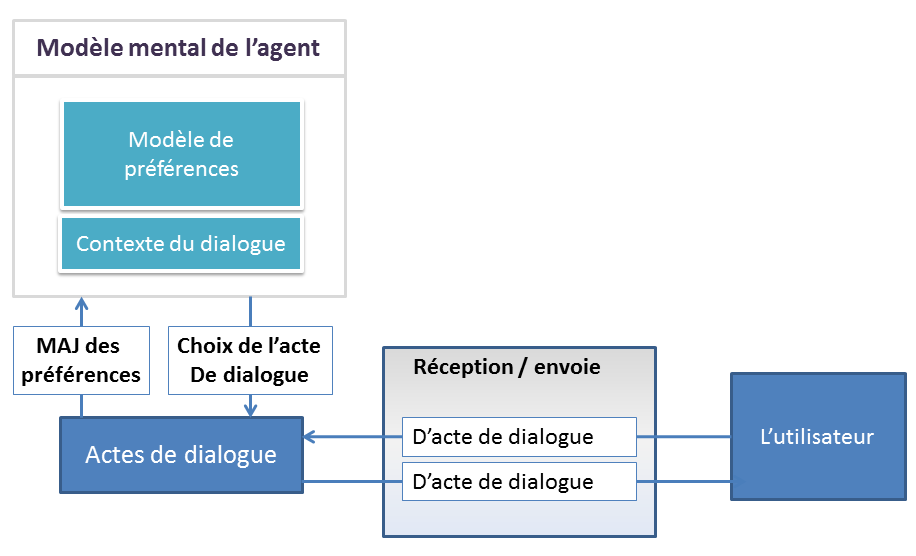
\includegraphics [width=4in]{figs/modele}}}
%	\vskip 8pt
%	\defig{modele}{Architecture du modèle de dialogue.}
%\end{figure}

\subsubsection{L'état mental}
\par La représentation actuelle de notre modèle vise a représenter une négociation coopérative entre l'agent et l'utilisateur. Afin de mener a bien la négociation, l'agent requiert une modélisation formelle de son environnement, à savoir ses préférences, ainsi que celles de l'utilisateur. Nous notons donc
 \begin{itemize}
 	\item  $\mathcal{P}_{self}$ le modèle de préférences de l'agent.
 	\item $\mathcal{P}_{other}$ le modèle de préférences de l'utilisateur que l'agent aura acquis durant le dialogue.
 	\item De plus; l'agent conserve les information qu'il communique à l'utilisateur (un module de la théorie d'esprit) qu'on note $\mathcal{P}_{other-about-self}$.
 \end{itemize}

 \par Dans ce qui suit, nous présenterons le modèle formelle de préférences utilisé pour la représentation de l'état mental de l'agent.
\\

\par \textbf{Le modèle de préférence :}
Le but principal de la négociation est de choisir une \emph{option} parmi un ensemble d'options qu'inclut le thème de la négociation (et donc de la conversation). Par exemple, pour une négociation sur le thème des ``Restaurants'', l'ensemble des options à choisir peut être : ``Chuck's cake'', ``The ducking Duck'', ``Ginza sushis''\ldots \\ On note donc $\mathcal{O}$, l'ensemble des options définis pour un thème de négociation. \par Afin de pouvoir  comparer ces options, les interlocuteurs se basent sur un ensemble de critères qui reflètent les caractéristiques de ces options. Par exemples, les critères de choix d'un restaurant sont \{la cuisine, le prix, l'ambiance, la localisation\}.  On note $\mathcal{C}$ les critères des options définis dans $\mathcal{O}$. Par ailleurs, chaque critère doit être mesurable de manière a pouvoir évaluer une option même qualitativement. Donc, $\forall$ \emph{c $\in\mathcal{ C}$},  on note \emph{D$_c$} son domaine de valeurs. par exemple, le domaine de valeurs du critère de la cuisine est noté $\emph{D}_{cuisine} = \{Chinois, Italien, Indien...\}$.

\par Chaque option $O\in \mathcal{O}$ définit une valeur pour chaque critère : 
$O = \{c_1=v_1,..., c_n=v_n\}$ avec $c_i \in \mathcal{C}, \forall i \in [1,n]$ et $v_i\in \emph{D}_{c_i}$. 
Par conséquent, on note $\{v(c,O) \in \emph{D}_{c} / \forall O \in \mathcal{O}, \forall c \in \mathcal{C}\}$ la valeur \emph{objective} du critère $c$ attribué à l'option $O$. La valeur objective d'un critère est indépendante des préférences; les interlocuteurs affectent les mêmes valeurs au critères d'une option indépendamment de leurs préférences. 
Par exemple, Ginza est un restaurant japonais coûteux : $v(prix, Ginza) = couteux $ et $(cuisine, Ginza) = japonais$. 

\par Nous présentons dans ce qui suit la représentation des préférences de l'agent qui lui permet d'exprimer et décider de ses préférences.
\\ \par \textbf{Représentation des préférences :}
Nous définissons une préférence \emph{P} comme une relation transitive et antisymétrique  définit sur un ensembles d'éléments \emph{A}, tel que:

\[ \left \{
\begin{array}{l}
\emph{P(a,b)} $ : \emph{a}  est préféré à $\emph{b}. \emph{ a,b} \in \emph{A}\\
\emph{P(b,a)} $:  \emph{b} est préféré à  $\emph{a}. \emph{ a,b} \in \emph{A}\\
$Sinon, aucune . $\\
\end{array}
\right .\]

Par exemple $P_{cuisine} (Japonais, Italien)$ signifie que l'interlocuteur préfère la cuisine japonaise à l'italienne. 

\par Nous définissons des variantes pour la notion de préférences:
\begin{itemize}
	\item  \emph{P(a,*)}  = \{$\forall$ \emph{x}$\in$\emph{A}, \emph{P(a,x)}\}, représente le fait que  \emph{a} est l'élément  \textit{le plus préféré} dans \emph{A}.
	\item Par opposition, \emph{P(*,b)} = \{$\forall$ \emph{x}$\in$\emph{A}, \emph{P(x,b)}\} signifie que \emph{b} est l'élément \textit{le moins préféré} dans l'ensemble \emph{A}. 
\end{itemize}


\par Notre but est de définir des préférences sur les options de la négociation.  Nous retrouvons dans la littérature plusieurs méthodes de calcul des préférences d'une option \cite{dodgson2009multi}. Ces méthodes nommées décision multi-critères calculent les préférences d'une option selon les performances de cette dernière sur l'ensemble des critères qui la définissent. Dans l'ensemble\cite{dodgson2009multi}, le calcul des préférences d'une option est fait par inférence à partir des préférences enregistrées sur les valeurs de ses critères. Cette inférence peut être réalisée grâce à différentes méthodes comme la fonction de somme pondérée \cite{yager2012ordered} ou encore les intégrales de Choquet \cite{chouquet1953}. \\

\par  \textbf{Sélection basée sur les préférences :} Une fois que le modèle de préférences est définit avec les relations de préférences sur les valeurs des critères, l'agent dispose d'information suffisantes pour pouvoir comparer deux options et calculer la relation 
$P(O_1, O_2) / O_1, O_2 \in \mathcal{O} $.

La relation de préférence entre deux options est effectuée en calculant l'utilité de chaque option grâce a une fonction de décision multi-critères. 
Nous avons sélectionné pour notre modèle la fonction de somme pondérée \cite{yager2012ordered} qui offre une méthode d'agréger les préférences sur les valeurs des critères calculé individuellement afin d'obtenir un score d'utilité globale pour l'option.
 
\par On note  $score(a)$ le nombre des successeurs de  $a$  dans le modèle de préférence $\mathcal{P}$, ce qui signifie que $|\{x \in \mathcal{D} / (a,x) \in \mathcal{P}\}|$. 
$rang(a)$ est le score normalisé $a$, qui est calculé en triant les valeurs d'un domaine $\mathcal{D}$ par ordre croissant de leurs scores. 


Par conséquent, calculer l'utilité d'une option grace à la fonction de somme pondéré est effectué comme suit:

\[U(O) = \sum_{c_j \in \mathcal{C}}  rang_R(c_j) \times score\left( v(O, c_j) \right) \] 


\par La relation de préférence entre deux options est donc calculée en comparant leurs utilités. 
\[ P(O_1, O_2)  = \left \{
\begin{array}{l}
P(O_1, O_2)$ \textit{if}  $U(O_1) > U(O_2) \\
P(O_2, O_1)$  \textit{if}  $U(O_2) > U(O_1) \\
$  \textit{aucune n'est préférée}  $U(O_2) = U(O_1)\\
\end{array}
\right .\]

 \par \textbf{Exemple de décision}

On suppose que l'agent cherche à calculer la relation de préférence suivante:  P(Clementine, Mogoroko), tel que 
\{Mogoroko, Clementine\} $\in$ Restaurant. La description des restaurants: 
\begin{itemize}
	\item Clementine=(Cuisine =\textit{Français}, Cost=\textit{Couteux}, Location=\textit{Paris02},
	\\Ambiance=\textit{Calme}).
	\item Mogoroko=(Cuisine=\textit{Japonais}, Cost=\textit{Abordable}, Location=\textit{Paris09}, 
	\\Ambiance=\textit{Calme}).
\end{itemize}

L'utilité de chaque option est calculée comme suit:
\begin{itemize}
	\item U(Clementine)=$rang$(Cuisine)$\times score$(\textit{Français})+$rang$(Prix)$\times score$(\textit{Couteux})\\+$rang$(Localisation)$\times score$(\textit{Paris02})
	+$rang$(Ambiance)$\times score$(\textit{Calme}).
	\item U (Mogoroko)= $rang$(Cuisine)$\times score$\textit{Japonais}+$rang$(Prix)$\times score$(\textit{Abordable})\\+$rang$(Localisation)$\times score$(\textit{Paris09}) +  
	$rang$(Ambiance)$\times score$(\textit{Calme})..
\end{itemize}
Le résultat du calcul des utilités: U(Clementine)=-3 and U(Mogoroko)=5.
\\  On conclut donc que $P(Mogoroko, Clementine)$ est vraie.
(i.e Mogoroko est préféré à Clementine).
\section{Conclusion et futurs travaux}
\label{conc}


\bibliographystyle{abbrv}
\bibliography{Library}

\end{document}
